\documentclass[letterpaper]{article} % DO NOT CHANGE THIS
\usepackage[submission]{aaai2027}  % DO NOT CHANGE THIS
\usepackage[hyphens]{url}  % DO NOT CHANGE THIS
\usepackage{graphicx} % DO NOT CHANGE THIS
\urlstyle{rm} % DO NOT CHANGE THIS
\def\UrlFont{\rm}  % DO NOT CHANGE THIS
\usepackage{natbib}  % DO NOT CHANGE THIS AND DO NOT ADD ANY OPTIONS TO IT
\usepackage{caption} % DO NOT CHANGE THIS AND DO NOT ADD ANY OPTIONS TO IT
\frenchspacing  % DO NOT CHANGE THIS

% Packages used by this paper
\usepackage{booktabs}
\usepackage{amsmath}
\usepackage{amssymb}

\pdfinfo{
/TemplateVersion (2027.1)
}

\setcounter{secnumdepth}{2} % numbered sections, lettered appendices

\newcommand{\idk}{``I don't know''}

\title{Does ``I Don't Know'' Track Knowledge or Popularity?\\Both, but Real-World Questions Cannot Say Which Matters More}
\author{
    Anonymous Submission
}
\affiliations{
}

\begin{document}

\maketitle

\begin{abstract}
When a language model says \idk, we would like that to mean it lacks the fact. We ask whether Llama-3.1-8B-Instruct's \idk{} follows whether it knows a fact or how popular the entity is. We split questions from the PopQA dataset by entity popularity (bottom vs.\ top tenth of Wikipedia page views) and by whether Llama answers them correctly. Popularity matters whether or not Llama knows the fact. On facts it does not know, it says \idk{} in 0.71 of replies for obscure entities and 0.18 for popular ones; on facts it answers correctly, 0.61 and 0.003. The effect of popularity holds across the whole popularity range (4,376 questions), and a second model, Gemma-2-9B-it, shows it on the same questions when the prompt invites abstaining. Over all questions together, the margin favors popularity, but its interval includes zero when whole relations are resampled. But the obscure facts Llama knows come almost entirely from three types of fact (capital, country and sport: 80 of 87). Comparing within a single type of fact, possible for country, composer and sport, gives no single answer: the point estimate favors popularity for country and knowledge for the two smaller types. Questions about real entities therefore cannot settle which factor matters more. Tests of the model's internals do not show that a sense of familiarity explains the popularity effect. So \idk{} depends on popularity as well as knowledge, and evaluations that read it as a report of missing knowledge should compare questions within the same type of fact and across popularity levels.
\end{abstract}

\section{Introduction}

Saying \idk{} when a fact is missing, instead of guessing, avoids a common source of hallucination \citep{kalai2025hallucinate}. Evaluations often read it that way, as a report that the model lacks the fact. Whether that reading holds depends on what the statement responds to. Model confidence is usually measured from the model's answers \citep{kadavath2022know,kuhn2023semantic}, but what a model says about its uncertainty and what its answers show can diverge \citep{ji2025calibrating}.

One alternative is familiarity with the entity asked about. In people, the feeling of being able to answer depends on how familiar a question's terms are, not only on whether the answer can be retrieved \citep{reder1992feeling,koriat2001combined}. In language models, internal signals that fire for entities the model knows suppress a default ``can't answer'' response, and \citet{lindsey2025biology} propose that a familiar name can trigger them when the fact is missing. If so, \idk{} should depend on familiarity separately from knowledge. The account also makes a sharper prediction. Where familiarity and knowledge disagree, abstention should follow familiarity: models should rarely abstain on familiar entities whose facts they lack, and often on unfamiliar entities whose facts they know.

Testing this requires separating familiarity from knowledge, which usually move together: an entity counts as known when the model answers about it correctly \citep{ferrando2025entity}. We use Wikipedia page views as a measurable stand-in for familiarity and cross them with knowledge taken from the model's own answers. We answer three questions in order: does popularity affect \idk{} (Section~\ref{sec:popularity}); does it matter more than knowledge, as the sharper prediction says (Section~\ref{sec:margin}); and does a sense of familiarity inside the model explain the popularity effect (Section~\ref{sec:familiarity})?

\paragraph{Main Contributions.}
\begin{enumerate}
\item \textbf{Popularity Affects Abstention at Both Knowledge Levels:} in Llama-3.1-8B-Instruct, obscure entities draw more \idk{} replies whether or not the model knows the fact (within relations, the known-fact part rests mainly on one relation).
\item \textbf{Real-World Questions Cannot Say Which Factor Matters More:} over all questions the margin favors popularity, but obscure known facts cluster in a few types of fact, the margin's interval includes zero when whole relations are resampled, and within types the comparison goes both ways.
\item \textbf{No Familiarity Explanation Found:} recognition, steering and lens tests do not show that familiarity explains the popularity effect.
\end{enumerate}

\section{Design}

\paragraph{Questions \& Labels.}
PopQA \citep{mallen2023popqa} groups its questions into 16 \emph{relations}, each a type of fact, such as a country's capital or an athlete's sport. Within each relation, subjects in the bottom and top tenth of page views form the \emph{obscure} and \emph{popular} groups. Knowledge comes from Llama's own answers, adapting \citet{gekhman2024finetuning}. We prompt with the chat template plus the start of the reply ``The answer is'' (the \emph{forced-answer prompt}), and grade a greedy answer and ten samples ($T = 0.7$) against the gold answers. A fact is \emph{known} if the greedy answer and at least 9 samples are correct, and \emph{unknown} if neither the greedy answer nor any sample is. This leaves 2,303 questions.

\begin{table}[t]
\centering
\small
\setlength{\tabcolsep}{1.3mm}
\begin{tabular}{@{}lcccc@{}}
\toprule
 & \multicolumn{2}{c}{Obscure} & \multicolumn{2}{c}{Popular} \\
\cmidrule(lr){2-3}\cmidrule(l){4-5}
 & known & unknown & known & unknown \\
\midrule
Says \idk & 0.61 & 0.71 & 0.00 & 0.18 \\
Questions & 87 & 100 & 100 & 100 \\
Entropy (nats) & 0.95 & 3.51 & 0.86 & 2.58 \\
\bottomrule
\end{tabular}
\caption{Llama-3.1-8B-Instruct by cell: share of free replies both judges label \idk, and first-answer-token entropy (intervals in Appendix~\ref{app:robust}).}
\label{tab:cells}
\end{table}

\paragraph{Abstention.}
We ask each question with the chat template alone (the \emph{free prompt}). For up to 100 questions in each of the four popularity $\times$ knowledge cells (387 in total), we draw three replies ($T = 0.7$, up to 96 tokens). A reply counts as \idk{} when two LLM judges (Qwen2.5-32B-Instruct, Gemma-2-27B-it) both label it so. Their agreement, Cohen's $\kappa = 0.91$ [0.88, 0.94], is above our pre-specified bar of 0.60 across the whole interval. (These labels correct an earlier faulty run of the Gemma judge; Appendix~\ref{app:judge}.) As a second measure covering every question, a regex detector scores 20 short replies (up to 24 tokens) for each of the 2,303 questions. Neither measure is validated against human labels.

\paragraph{Effects.}
The \emph{popularity effect} is obscure minus popular abstention, averaged over the two knowledge levels; the \emph{knowledge effect} is unknown minus known, averaged over the two popularity levels. Both are positive when obscurity or missing knowledge raises abstention. Their difference is the \emph{popularity margin}: positive when abstention follows popularity more than knowledge. Intervals are 95\% bootstrap intervals from resampling questions within each cell. Each analysis followed a plan recorded before it ran, except those marked \emph{post hoc} (chosen after seeing data). The primary measure was itself adopted after an earlier measure was seen (Appendix~\ref{app:robust}).

\section{Popularity Affects Abstention at Both Knowledge Levels}
\label{sec:popularity}

\begin{figure*}[t]
\centering
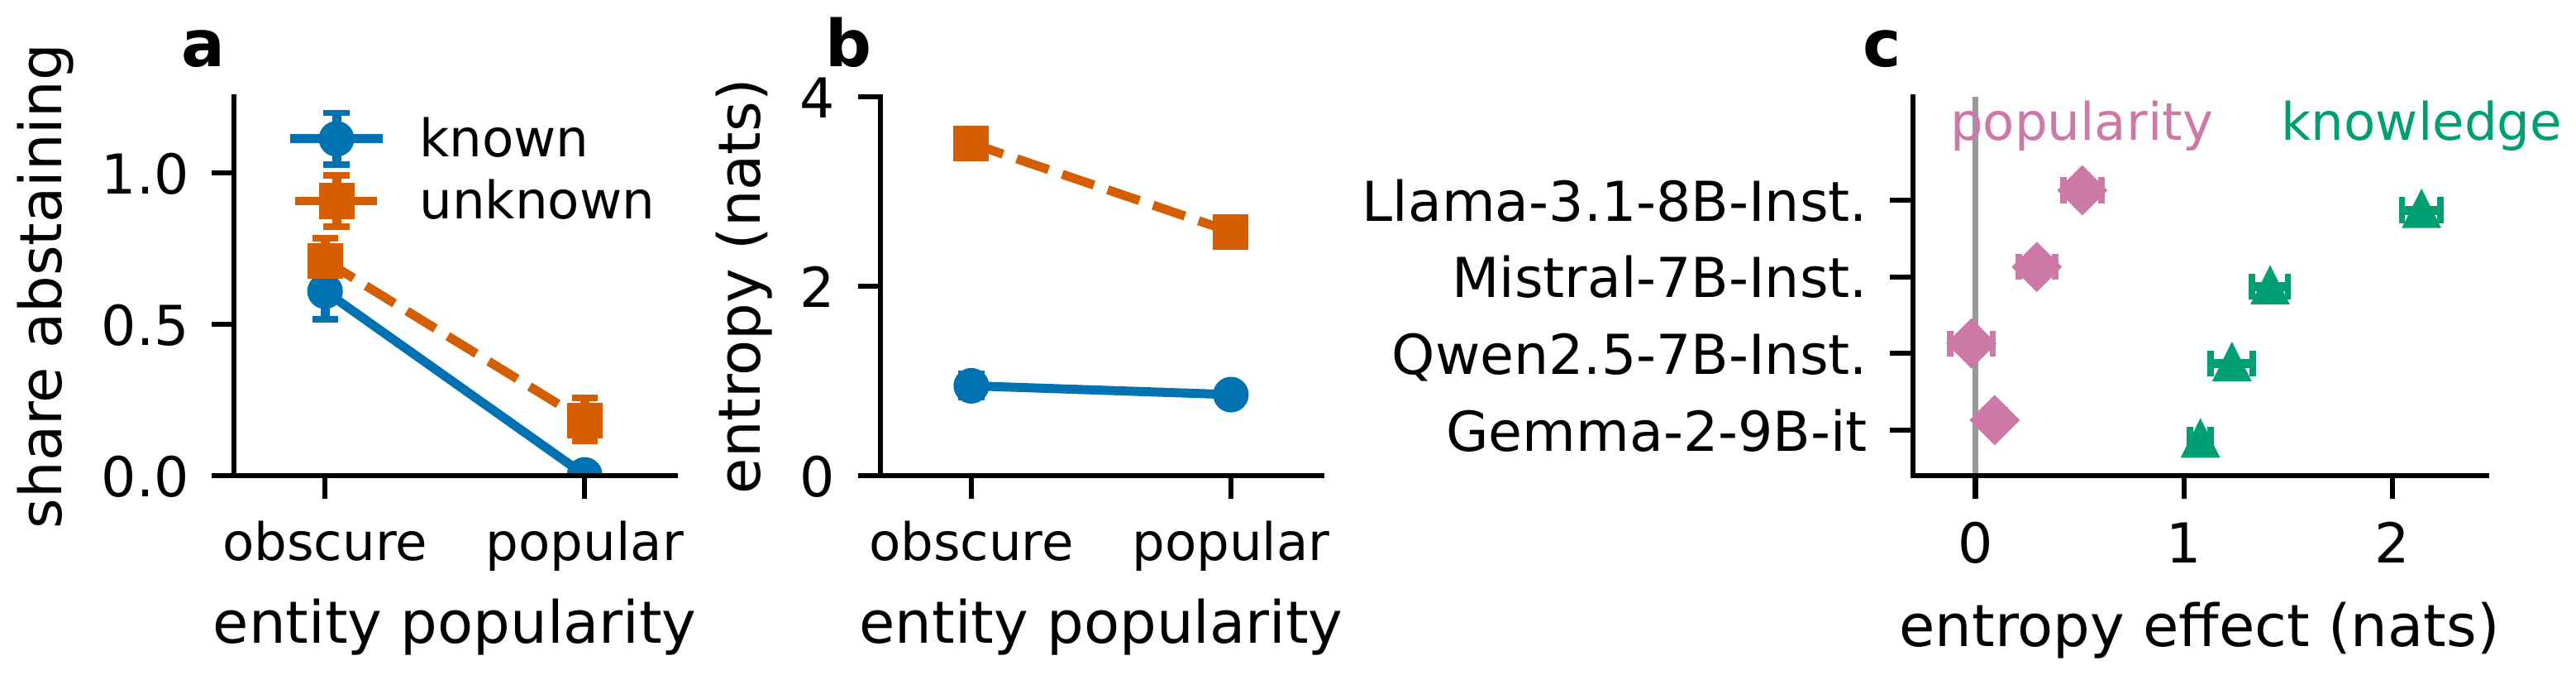
\includegraphics[width=0.8\textwidth]{figures/fig1}
\caption{In Llama, abstention falls with popularity at both knowledge levels; answer entropy, a control, follows knowledge much more than popularity. (a) Share of free replies both judges label \idk; (b) entropy of the first answer token after ``The answer is''; (c) popularity and knowledge effects on that entropy in four instruct models. 95\% bootstrap intervals.}
\label{fig:cells}
\end{figure*}

Table~\ref{tab:cells} and Figure~\ref{fig:cells}a give the four cells. Among facts Llama does not know, it says \idk{} in 0.71 of replies on obscure entities and 0.18 on popular ones, a gap of $+0.53$ [$+0.42$, $+0.63$] (post hoc). The gap shrinks to $+0.35$ [$+0.19$, $+0.50$] after three corrections to the knowledge labels (Appendix~\ref{app:robust}; post hoc) but stays positive. Among facts it answers correctly, the rate is 0.61 on obscure entities and, by the judges, 0.003 (one of 300 sampled replies) on popular ones. These are genuine declines rather than hidden answers: at most 0.02 of \idk{} replies in any cell contain the gold answer (post hoc, not counting answers that merely repeat the subject's name).

As a control, we measure how unsure Llama is of its answer: the entropy of the first answer token after ``The answer is''. It follows knowledge much more than popularity (Figure~\ref{fig:cells}b; panel c shows the same in four instruct models). In the two known cells it is similar (0.95 vs.\ 0.86 nats), so the gap between them is not explained by how sure Llama is of its answer.

\paragraph{The Whole Popularity Range.}
The design so far compares the extreme tenths. We therefore drew up to 300 questions per relation, spread evenly over the ten popularity tenths within it (4,376 questions, all 16 relations; three have fewer than 300), and regressed abstention on popularity rank and a knowledge score, the share of ten forced answers that are correct, with relation fixed effects (fractional logit; the plan was recorded before the run, with one dated amendment). Obscurity raises abstention: from the most to the least viewed question of a relation the coefficient is $+3.68$ [$+2.73$, $+4.74$] (relations resampled). Averaged over all questions, predicted abstention is 0.21 at the 90th percentile of popularity and 0.73 at the 10th. The coefficient is $+3.56$ [$+2.54$, $+4.74$] without the extreme tenths, $+3.42$ [$+2.46$, $+4.58$] without country, capital and sport, and $+4.41$ [$+3.32$, $+5.68$] with the regex. Knowledge lowers abstention ($-0.97$ [$-1.62$, $-0.42$]); we do not rank the two coefficients, because their sizes depend on how the two variables are scaled (Appendix~\ref{app:range}).

\paragraph{A Second Model.}
We repeated this check on Gemma-2-9B-it with the same questions, asked with the prompt that invites abstaining because Gemma rarely says \idk{} without it (Appendix~\ref{app:other}); knowledge is Gemma's own, and the plan was recorded before the run. Obscurity again raises abstention: $+2.99$ [$+2.35$, $+3.82$], $+2.56$ [$+1.85$, $+3.49$] without the extreme tenths and $+3.16$ [$+2.50$, $+3.91$] with the regex. Predicted abstention is 0.15 at the 90th percentile of popularity and 0.47 at the 10th. The prompts differ between the two models, so the sizes are not comparable. The popularity effect thus holds for Llama-3.1-8B-Instruct and Gemma-2-9B-it on PopQA.

So popularity affects when Llama says \idk. Because obscure known facts cluster in a few relations, the next section checks this within relations, as part of asking how popularity compares with knowledge.

\section{The Overall Margin Favors Popularity, but Within Relations the Answer Differs}
\label{sec:margin}

Over all questions together, the popularity effect on abstention is $+0.57$ [$+0.50$, $+0.63$] and the knowledge effect $+0.14$ [$+0.07$, $+0.21$], a popularity margin of $+0.43$ [$+0.31$, $+0.54$]. The margin stays positive under other judges and labels, though it shrinks under some (Table~\ref{tab:robust}). It repeats with fresh replies ($+0.45$ [$+0.34$, $+0.56$]). Llama might guess some obscure facts from the name alone, so we removed those it still answers when the name is misspelled; the margin is then $+0.50$ [$+0.37$, $+0.63$]. When the prompt invites abstaining, Gemma-2-9B, Qwen2.5-7B and Mistral-7B also give positive margins and OLMo-2-7B does not (Appendix~\ref{app:other}).

Yet the margin compares cells that hold different kinds of question. In this design it equals abstention on obscure known facts minus abstention on popular unknown facts, because the other two cells cancel. Llama knows few obscure facts: 80 of the 87 come from three relations (capital, country, sport), while only 4 of the 100 popular unknown questions do. Outside those three relations the margin is $-0.05$ [$-0.25$, $+0.27$], from only 7 obscure known facts (post hoc). If whole relations, rather than questions, are resampled, the interval for the overall margin widens to [$-0.15$, $+0.62$].

\begin{table}[t]
\centering
\small
\setlength{\tabcolsep}{1.2mm}
\begin{tabular}{@{}lrl@{}}
\toprule
Difference in abstention & All & Within relations \\
\midrule
Obscure $-$ popular, known & $+0.65$ & $+0.28$ [$+0.21$, $+0.37$] \\
Obscure $-$ popular, unknown & $+0.61$ & $+0.44$ [$+0.29$, $+0.59$] \\
Unknown $-$ known, obscure & $+0.17$ & $+0.48$ [$+0.38$, $+0.58$] \\
Unknown $-$ known, popular & $+0.21$ & $+0.32$ [$+0.19$, $+0.47$] \\
\midrule
Popularity margin & $+0.44$ & $-0.04$ [$-0.20$, $+0.11$] \\
\bottomrule
\end{tabular}
\caption{Holding the relation fixed, regex measure on all 2,303 labeled questions. All: every relation together. Within: mean over the three relations with at least 3 questions in every cell (country, composer, sport), resampling questions within relation and cell. Post hoc.}
\label{tab:within}
\end{table}

To compare the factors directly, we hold the relation fixed (Table~\ref{tab:within}). Only the regex measure covers enough questions for this; on it, the margin over all questions is $+0.44$, close to the judges' $+0.43$. Only three relations have at least three questions in every cell: country, composer and sport. They overlap with, but are not the same as, the three that hold most obscure known facts. Averaged over them, popularity and knowledge have similar effects, and the margin is $-0.04$ [$-0.20$, $+0.11$]. The average hides opposite results. In country, the only relation with at least ten questions in every cell and home to most obscure known facts, the margin is $+0.69$ (a point estimate), larger than over all questions. In composer and sport, whose obscure known cells are tiny, it is $-0.60$ and $-0.21$. Popularity's effect on known facts within relations also comes almost entirely from country.

So the overall margin mixes relations, and holding the relation fixed does not give one answer. Questions about real entities cannot settle whether popularity outweighs knowledge, because the questions that would decide it, obscure facts the model knows, exist in only a few relations. What they do show is that popularity matters alongside knowledge. That leaves the question of what the popularity effect is.

\section{No Familiarity Signal Found to Explain the Popularity Effect}
\label{sec:familiarity}

If the popularity effect is familiarity, Llama should register obscure names as unfamiliar, and that signal should account for the effect. We test this three ways.

\paragraph{Recognition.}
We asked Llama to describe each entity, and Llama-3.3-70B graded the description against Wikidata. Recognition rises with page views (rank correlation $+0.52$; among unknown facts 0.11 obscure vs.\ 0.56 popular), so Llama does register obscure names as less familiar. But controlling for recognition reduces the popularity effect on abstention by only 4\%.

\paragraph{Steering.}
We added fixed vectors to the model's hidden states \citep{arditi2024refusal}. The vector from popular toward obscure questions raises abstention, but it points almost the same way as a vector that triggers abstention, fitted on popular questions alone (cosine similarity 0.89). After subtracting that shared part, it raises abstention by only $+0.01$ [$-0.00$, $+0.02$] more than random vectors (Appendix~\ref{app:other}). Such steering effects do not show that a model uses a signal in normal operation \citep{che2026feature}, so this neither shows nor rules out a familiarity signal earlier in the model.

\paragraph{Lens.}
Reading out the middle layers of four base models with Jacobian lenses \citep{gurnee2026verbalizable} shows obscurity and missing knowledge both raising the score of hedging words such as ``not'' and ``unknown'' (Appendix~\ref{app:other}). This shows both factors at work but does not show where the instruct model's behavior arises.

So Llama registers obscure names as less familiar, but none of the three tests shows that this explains the popularity effect.

\section{Conclusion}

We asked whether Llama's \idk{} follows knowledge or popularity. It follows both: obscurity raises abstention whether or not the model knows the fact (within relations, for known facts, mainly in one relation), and so does missing knowledge. Which matters more cannot be settled with questions about real entities. The overall margin favors popularity, but it compares obscure facts in a few relations with popular facts in others, and within relations the answer differs, because obscure facts a model knows are rare outside a few types of fact. Llama does register obscure names as less familiar, but that signal does not explain the popularity effect, and page views also carry other properties of names, so the effect's cause remains to be shown. Both open points call for the same design: assigning familiarity and knowledge at random, for example by training on invented entities. For evaluation, the practical point is that Llama's abstention rate measures more than missing knowledge, and it should be compared within relations and across popularity levels.

\section*{Limitations}

We study one model in depth and a second in one check, under a prompt that invites abstaining, on one dataset; other models appear only in Figure~\ref{fig:cells}c and Appendix~\ref{app:other}. Abstention is scored by LLM judges and a regex, neither validated against human labels, and their errors could differ by cell. Knowledge labels come from a single forced-answer prompt and transfer imperfectly to other prompts. The within-relation comparison rests on three relations (country, composer, sport) with small cells and on the regex measure. The main design contrasts the extreme tenths of popularity; the whole-range check is a regression in which knowledge is graded by string match. Judge agreement is agreement between two LLMs. Several analyses were chosen after seeing data and are marked post hoc. Page views stand in for familiarity and also carry other properties of names. The Gemma-2 lens runs (Table~\ref{tab:lens}) and the steering runs on Gemma-2, which we do not report, were done before the attention fix and were not rerun with the corrected implementation; the steering results here are on Llama. The overall margin depends on which relations are included: 80 of the 87 obscure known facts come from three relations, and its interval includes zero when whole relations are resampled ([$-0.15$, $+0.62$]). The analysis plans were recorded by the authors before each run (file hashes and times we recorded ourselves; commit times precede the runs only for the whole-range checks), so the record is not independently timestamped. The correction of the Gemma judge labels was made after the first runs, so it is post hoc, although it fixes an implementation bug and we report both sets of numbers (Appendix~\ref{app:judge}). The replication covers one more model (Gemma-2-9B-it) with one prompt; the full-range result is for Llama-3.1-8B-Instruct and Gemma-2-9B-it on PopQA, not for other model families or datasets.

\bibliography{references}

%=====================================================================
% Technical appendix (supplementary material)
%=====================================================================
\appendix

\section{The Overall Margin Under Other Measures and Labels}
\label{app:robust}

\begin{table}[!ht]
\centering
\small
\begin{tabular}{@{}p{0.52\columnwidth}l@{}}
\toprule
Variant & Margin \\
\midrule
Two judges (primary; adopted post hoc) & $+0.43$ [$+0.31$, $+0.54$] \\
Three judges, majority & $+0.43$ [$+0.31$, $+0.54$] \\
Regex on the judged replies (post hoc) & $+0.43$ [$+0.30$, $+0.55$] \\
One judge, corrected & $+0.13$ [$+0.02$, $+0.24$] \\
Fresh replies & $+0.45$ [$+0.34$, $+0.56$] \\
New questions, 10th--30th vs.\ 70th--90th percentile & $+0.15$ [$+0.03$, $+0.26$] \\
Name-guessable facts removed & $+0.50$ [$+0.37$, $+0.63$] \\
Unknown facts regraded by meaning & $+0.35$ [$+0.22$, $+0.48$] \\
Three label corrections (post hoc) & $+0.24$ [$+0.07$, $+0.41$] \\
\bottomrule
\end{tabular}
\caption{Llama's overall popularity margin under other measures and labels. The primary two-judge measure was adopted after the corrected one-judge measure ($+0.13$) was seen. After the three label corrections, the unknown-fact gap is $+0.35$ [$+0.19$, $+0.50$]. Cell intervals for Table~\ref{tab:cells}: obscure known [0.52, 0.70], obscure unknown [0.63, 0.79], popular known [0.00, 0.01], popular unknown [0.12, 0.26].}
\label{tab:robust}
\end{table}

\section{Correction of One Judge}
\label{app:judge}

The labels of the Gemma-2-27B judge in an earlier version of this paper came from an incorrect forward pass: the default attention implementation of the transformers library (sdpa) omits the attention soft-capping that Gemma-2 uses. We found this in a later experiment, after the results above had been seen, so the correction is post hoc. The stored labels are reproduced exactly with that implementation; with eager attention, and with vLLM, the labels agree with each other on all 1,161 Llama replies and differ from the stored ones. We relabeled all 49,521 stored replies with the same prompt and parser and kept the rule that both judges must say DONT\_KNOW. The two-judge agreement on Llama rose from $\kappa = 0.62$ to 0.91, the margin from $+0.30$ [$+0.20$, $+0.40$] to $+0.43$ [$+0.31$, $+0.54$], and the unknown-fact gap from $+0.34$ [$+0.25$, $+0.43$] to $+0.53$ [$+0.42$, $+0.63$] (after the label corrections, from $+0.18$ [$+0.04$, $+0.31$] to $+0.35$ [$+0.19$, $+0.50$]). Agreement between two LLM judges is not validation against people. Gemma-2-9B as a tested model was run with the same implementation; on 300 questions its forced answers were equally correct and its entropies nearly identical ($r = 0.999$) with the correct one. Its steering and lens runs were not rerun.

\section{The Whole Popularity Range}
\label{app:range}

\begin{table*}[!t]
\centering
\small
\begin{tabular}{@{}lrll@{}}
\toprule
 & $n$ & Two judges & Regex \\
\midrule
\multicolumn{4}{@{}l}{\emph{Llama-3.1-8B-Instruct}} \\
All tenths & 4,376 & $+3.68$ [$+2.73$, $+4.74$] & $+4.41$ [$+3.32$, $+5.68$] \\
Tenths 2 to 9 & 3,501 & $+3.56$ [$+2.54$, $+4.74$] & $+4.15$ [$+2.99$, $+5.49$] \\
W/o three rel. & 3,476 & $+3.42$ [$+2.46$, $+4.58$] & $+4.10$ [$+2.99$, $+5.52$] \\
Know.\ 11 levels & 4,376 & $+3.73$ [$+2.76$, $+4.82$] & $+4.44$ [$+3.34$, $+5.72$] \\
\midrule
\multicolumn{4}{@{}l}{\emph{Gemma-2-9B-it, inviting prompt}} \\
All tenths & 4,342 & $+2.99$ [$+2.35$, $+3.82$] & $+3.16$ [$+2.50$, $+3.91$] \\
Tenths 2 to 9 & 3,474 & $+2.56$ [$+1.85$, $+3.49$] & $+2.75$ [$+2.11$, $+3.54$] \\
W/o three rel. & 3,442 & $+3.01$ [$+2.27$, $+3.90$] & $+3.27$ [$+2.52$, $+4.06$] \\
Know.\ 11 levels & 4,342 & $+3.03$ [$+2.38$, $+3.87$] & $+3.20$ [$+2.57$, $+3.92$] \\
\bottomrule
\end{tabular}
\caption{Coefficient of obscurity (0 for the most viewed question of a relation, 1 for the least viewed) on abstention, with the knowledge score and relation fixed effects; fractional logit, 95\% intervals resampling whole relations (5,000 draws). Three relations (W/o three rel.): country, capital, sport. Know.\ 11 levels: knowledge in 11 levels. With the uncorrected labels of the Gemma judge the first two-judge entry is $+2.41$ [$+1.74$, $+3.22$]. Gemma: the relation color (34 questions) has no abstention and is dropped from the fits; 26 draws of the 11-level two-judge fit and 1 of the regex fit did not converge and are dropped.}
\label{tab:range}
\end{table*}

\begin{figure}[!ht]
\centering
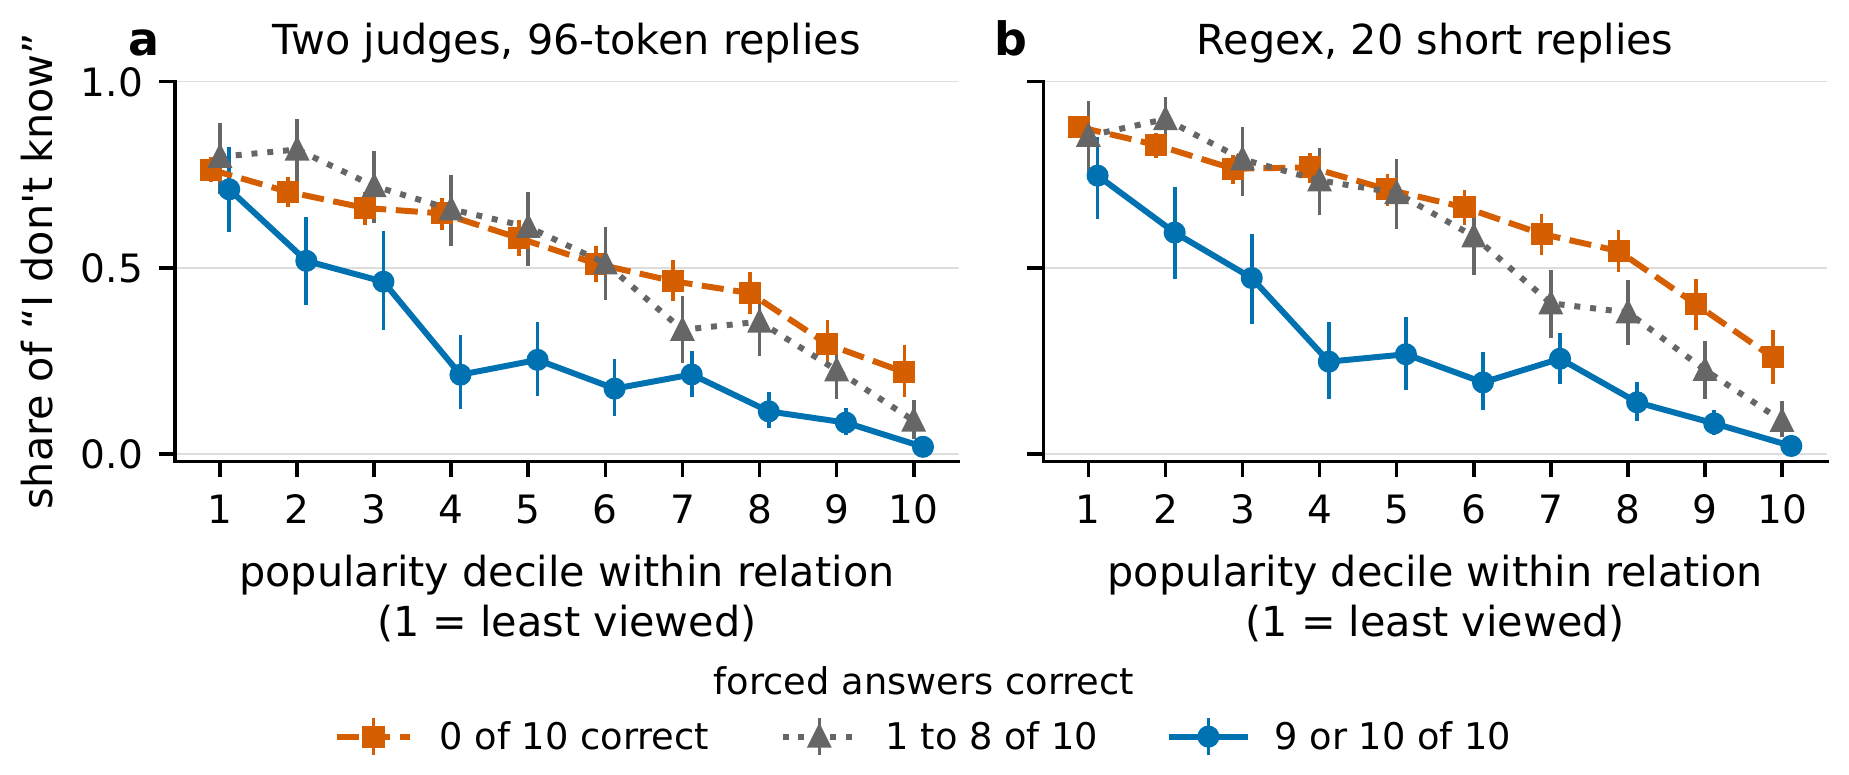
\includegraphics[width=\columnwidth]{figures/fig2}
\caption{Share of \idk{} replies by popularity tenth, for questions with 0, 1 to 8, and 9 or 10 of 10 forced answers correct. 95\% intervals resample questions.}
\label{fig:range-llama}
\end{figure}

\begin{figure}[!ht]
\centering
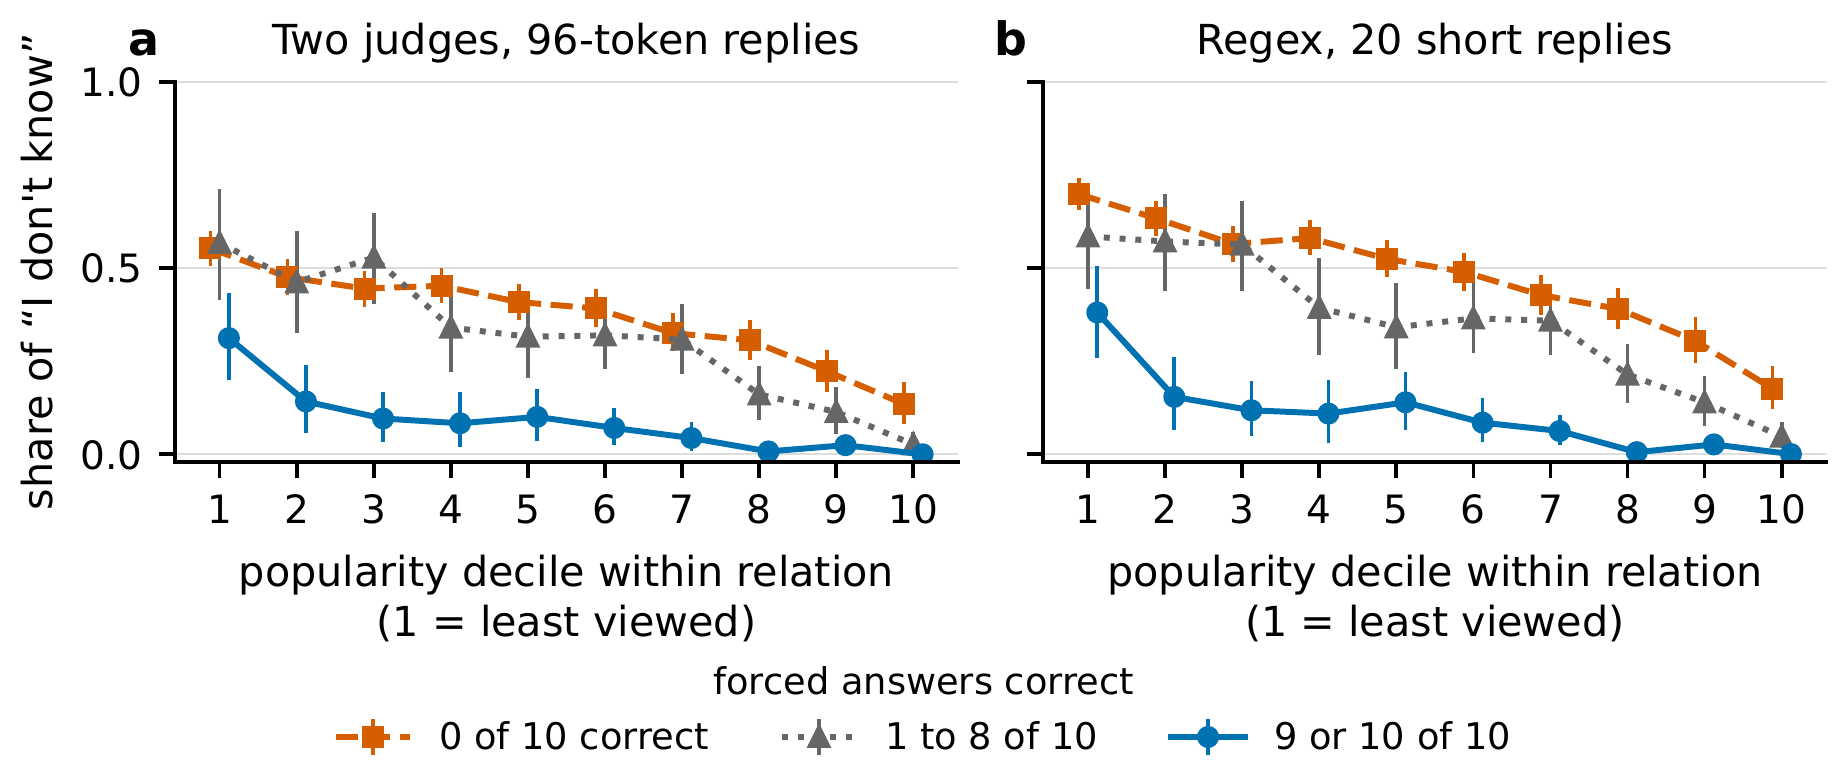
\includegraphics[width=\columnwidth]{figures/fig3}
\caption{As Figure~\ref{fig:range-llama}, for Gemma-2-9B-it with the prompt that invites abstaining.}
\label{fig:range-gemma}
\end{figure}

For Llama, the amendment replaced two pilot checks, after the pilot and before the full run, when the pilot revealed the judge fault (Appendix~\ref{app:judge}); sample, prompts, model and decision rules were unchanged. Replies were generated with vLLM. The knowledge score and the paper's known/unknown labels come from the same forced-answer prompt and string grader. The Gemma run used the same questions, judges and analysis and needed no amendment; knowledge lowers abstention there too ($-1.81$ [$-2.28$, $-1.49$]). One judge, Gemma-2-27B, is from the tested model's family; with Qwen alone the obscurity coefficient is $+3.12$ [$+2.50$, $+3.84$]. Table~\ref{tab:range} and Figures~\ref{fig:range-llama} and~\ref{fig:range-gemma} give the details.

\section{Other Models, Steering and Lens}
\label{app:other}

\paragraph{Other Models.}
On the free prompt, Qwen2.5-7B, Gemma-2-9B and Mistral-7B rarely say \idk{} by the judges' labels; three judges agree on Gemma and Mistral (Fleiss $\kappa = 0.94$ and 0.75) and fall just short of the bar on Qwen (0.59). Ending each question with ``If you do not know the answer, say that you do not know'' raises abstention. Three judges then agree on all five models (Fleiss $\kappa$: Llama 0.97, Gemma 0.89, Qwen 0.74, Mistral 0.80, OLMo-2-7B 0.86). The margins are $+0.47$ [$+0.35$, $+0.59$] for Llama, $+0.30$ [$+0.19$, $+0.40$] for Gemma, $+0.16$ [$+0.01$, $+0.31$] for Qwen and $+0.17$ [$+0.06$, $+0.28$] for Mistral; for OLMo-2-7B the interval includes zero ($-0.09$ [$-0.21$, $+0.04$]).

\paragraph{Steering.}
Vectors were fitted on half of the questions at layer $\mathrm{round}(0.55(L-1))$ and the last position of the free prompt; the strength was chosen on a second set of popular known questions, and effects were scored on a third by a majority of three judges. The abstention vector was fitted on 63 abstaining against 548 answering popular questions. Compared with 20 random vectors, the abstention vector itself raises abstention by $+0.14$ [$+0.10$, $+0.19$], and the popular-to-obscure vector by $+0.16$ [$+0.12$, $+0.21$].

\paragraph{Lens.}
Effects at middle layers in base models (95\% intervals): the full readout compares hedging words with answer-opening words; the hedge term counts hedging words alone (Table~\ref{tab:lens}).

\begin{table*}[!ht]
\centering
\small
\begin{tabular}{@{}lllll@{}}
\toprule
 & \multicolumn{2}{c}{Full readout} & \multicolumn{2}{c}{Hedge term} \\
\cmidrule(lr){2-3}\cmidrule(l){4-5}
Model & Obscurity & Not knowing & Obscurity & Not knowing \\
\midrule
Llama-3.1-8B & $+0.67$ [$+0.59$, $+0.75$] & $+0.36$ [$+0.28$, $+0.44$] & $+0.55$ [$+0.46$, $+0.64$] & $+0.56$ [$+0.47$, $+0.65$] \\
Gemma-2-9B & $+0.39$ [$+0.34$, $+0.43$] & $+0.37$ [$+0.33$, $+0.42$] & $+0.28$ [$+0.21$, $+0.35$] & $+0.30$ [$+0.23$, $+0.37$] \\
Gemma-2-2B & $+0.40$ [$+0.33$, $+0.47$] & $+0.11$ [$+0.04$, $+0.18$] & $+0.10$ [$+0.03$, $+0.17$] & $+0.37$ [$+0.30$, $+0.43$] \\
OLMo-3-7B & $+0.29$ [$+0.19$, $+0.38$] & $-0.30$ [$-0.40$, $-0.20$] & $+0.61$ [$+0.53$, $+0.70$] & $+0.53$ [$+0.45$, $+0.62$] \\
\bottomrule
\end{tabular}
\caption{Lens effects in base models. Lenses are fitted per model, so compare within a model.}
\label{tab:lens}
\end{table*}

\end{document}
